
\documentclass{standalone}

%\documentclass[convert]{standalone}
% convert: in addition to pdf output files, png files are created
% convert options does work properly with -output-directory option of latexmk

\usepackage{tikz-feynman}
\tikzfeynmanset{compat=1.1.0}


\begin{document}
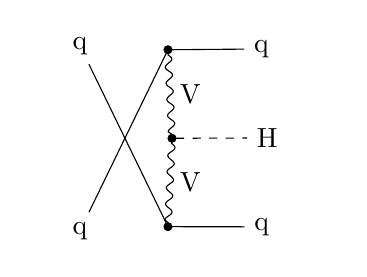
\begin{tikzpicture}
        \begin{feynman}
            % higgs production, VBF, u-channel

            % comment on layout:
            % similar layout to t-channel. Difference:
            % - line from qi1 to a, and qi2 to c are not drawn
            % - instead: in the \digram section, manual lines with a and c switched are drawn
            \diagram [small, vertical=a to c] {
            qi1 [particle=q]
            -- [draw=none] a [dot],
            a -- qf1 [particle=q],
            a -- [boson, edge label=V] b [dot],
            b -- [scalar] H [particle=H],
            b -- [boson, edge label=V] c [dot],
            qi2 [particle=q]
            -- [draw=none] c
            --  qf2 [particle=q],

            % invisible helper lines for layout
            qi1 -- [draw=none] ih1 -- [draw=none] qi2,
            qf1 -- [draw=none] fh1 -- [draw=none] fh2 -- [draw=none] qf2,
            qf1 -- [draw=none] H,
            H -- [draw=none] qf2,
            };

            \diagram* {
            (qi1) -- (c),
            (qi2) -- (a),
            };
        \end{feynman}
    \end{tikzpicture}
\end{document}
